\documentclass[xcolor=dvipsnames]{beamer}

\usepackage{amsmath, amssymb, graphicx}
\usepackage[english]{babel}
\usepackage{times}
\usepackage[utf8]{inputenc}
\usepackage[T1]{fontenc}
\usepackage{listings}
\usepackage{hyperref}
\usepackage[norelsize,ruled,vlined]{algorithm2e}
\usepackage{color}
\usepackage{hyperref}
\usepackage{booktabs}
\usepackage{tikz}
\usetikzlibrary{matrix}
\usetikzlibrary{arrows}
\usetikzlibrary{positioning}
\usetikzlibrary{shapes.multipart}

\newcommand{\fancyh}{\mathcal{H}}
\newcommand{\gangle}[1]{\langle{} #1 \rangle{}}
\newcommand{\myd}{\mathrm{d}}
\newcommand{\NN}{\mathbb{N}}
\newcommand{\RR}{\mathbb{R}}
\newcommand{\ZZ}{\mathbb{Z}}

\newsavebox{\flowgraph}
\savebox{\flowgraph}{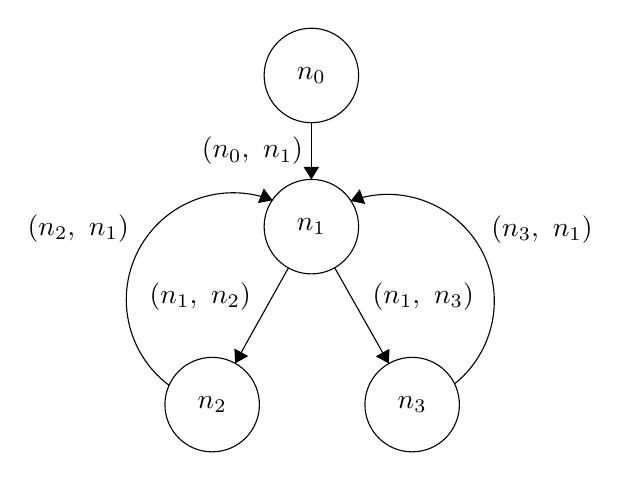
\begin{tikzpicture}[scale=0.2]
        \tikzstyle{every node}+=[inner sep=0pt]
        \draw [black] (24.7,-14) circle (3);
        \draw(24.7,-14) node {$n_0$};
        \draw [black] (24.7,-23.6) circle (3);
        \draw (24.7,-23.6) node {$n_1$};
        \draw [black] (18.4,-34.9) circle (3);
        \draw (18.4,-34.9) node {$n_2$};
        \draw [black] (31.1,-34.9) circle (3);
        \draw (31.1,-34.9) node {$n_3$};
        \draw [black] (15.682,-33.688) arc (-126.68179:-291.59948:6.793);
        \fill [black] (22.24,-21.93) -- (21.68,-21.17) -- (21.31,-22.1);
        \draw (13.14,-23.73) node [left] {$(n_2,\mbox{ }n_1)$};
        \draw [black] (27.192,-21.975) arc (110.40413:-51.35216:6.765);
        \fill [black] (27.19,-21.97) -- (28.12,-22.16) -- (27.77,-21.23);
        \draw (36.1,-23.76) node [right] {$(n_3,\mbox{ }n_1)$};
        \draw [black] (23.24,-26.22) -- (19.86,-32.28);
        \fill [black] (19.86,-32.28) -- (20.69,-31.82) -- (19.81,-31.34);
        \draw (20.89,-28.05) node [left] {$(n_1,\mbox{ }n_2)$};
        \draw [black] (26.18,-26.21) -- (29.62,-32.29);
        \fill [black] (29.62,-32.29) -- (29.66,-31.35) -- (28.79,-31.84);
        \draw (28.56,-28.03) node [right] {$(n_1,\mbox{ }n_3)$};
        \draw [black] (24.7,-17) -- (24.7,-20.6);
        \fill [black] (24.7,-20.6) -- (25.2,-19.8) -- (24.2,-19.8);
        \draw (24.2,-18.8) node [left] {$(n_0,\mbox{ }n_1)$};
    \end{tikzpicture}
}

\mode<presentation>
{% \setbeamertemplate{navigation symbols}{}
    % \setbeamertemplate{items}[ball]
    % \setbeamertemplate{blocks}[rounded][shadow=true]
    \beamertemplatenavigationsymbolsempty
    \usecolortheme[named=Sepia]{structure}
    \usetheme{Warsaw}
    \useoutertheme{infolines}
    \setbeamercovered{transparent}
}

\lstset{language = [LaTeX]TeX,
    % captionpos=b,
    basicstyle= \small \ttfamily,
    keywordstyle = \bfseries \color{blue},
    commentstyle = \color{green}
}

\definecolor{mygreen}{rgb}{0, 178, 115}

\tikzstyle{block} = [rectangle, draw, font=\tiny, text centered, rounded corners, minimum height=1em]
\tikzstyle{line} = [draw, -latex']
\tikzstyle{value} = [label, red, font=\tiny, thick, node distance=0.4cm]

\title[Monotone Data Flow Analysis Frameworks]{Monotone Data Flow Analysis Frameworks}
\author{Fengyun Liu, Ólafur Páll Geirsson}
\institute[EPFL]{}
\date{\today}


% Delete this, if you do not want the table of contents to pop up at
% the beginning of each subsection:
\AtBeginSection[]
{\begin{frame}<beamer>{Overview}
        \tableofcontents[
            sections={1-6},
            currentsection,
            currentsubsection,
            hideothersubsections,
            sectionstyle=show/shaded,
        subsectionstyle=show/shaded/hide]
    \end{frame}
}

\begin{document}


%%%%%%%%%%%%%%%%%%%%%%%%%%%%%%%%%%%%%%%%%%%%%%%%%%%%%%%%%%%%%%%
% 0. Titlepage
%%%%%%%%%%%%%%%%%%%%%%%%%%%%%%%%%%%%%%%%%%%%%%%%%%%%%%%%%%%%%%%
\begin{frame}
    \titlepage{}
\end{frame}
\begin{frame}{Today's agenda}
\tableofcontents[hideallsubsections,
    sections={2-6}
]
\end{frame}

%%%%%%%%%%%%%%%%%%%%%%%%%%%%%%%%%%%%%%%%%%%%%%%%%%%%%%%%%%%%%%%
% 1. Background
%%%%%%%%%%%%%%%%%%%%%%%%%%%%%%%%%%%%%%%%%%%%%%%%%%%%%%%%%%%%%%%
\section{Introduction} % (fold)
\section{Background} % (fold)
\label{sec:Background}

\subsection{Flow graph}\label{sec:flowgraph}
\begin{frame}[fragile]
    \frametitle{Flow graph}
    \begin{definition}
        A flow graph is a triple \alert{$G = (N, E, n_0)$}.
    \end{definition}
    \begin{columns}
        \begin{column}{0.3\textwidth}
            Example:
            $N = \{n_0, n_1, n_2, n_3\}$
            $E = \{(n_0, n_1)$,\\
            $(n_1, n_2),(n_1, n_3)$, $(n_2, n_1),(n_3, n_1)\}$
        \end{column}
        \begin{column}{0.7\textwidth}
            \begin{center}
                \usebox{\flowgraph}
            \end{center}
        \end{column}
    \end{columns}
\end{frame}
\subsection{Semilattice}
\begin{frame}[fragile]
    \frametitle{Set $L$ with \alert{meet} operation $\wedge$}
    \begin{align*}
        a \wedge a & = a & (idempotent) \\
        a \wedge b & = b \wedge a & (commutative) \\
        a \wedge (b \wedge c) & = (a \wedge b) \wedge c & (associative)
    \end{align*}
\end{frame}
\subsection{Semilattice: ordering}
\begin{frame}[fragile]
    \frametitle{The meet $\wedge$ defines an \alert{order} on $L$}
    \begin{align*}
        a & \geqq b & \text{iff } a \wedge b = b \\
        a > b & = b \wedge a & \text{iff } a \wedge b = b \text{\ and } a \neq b
    \end{align*}
\end{frame}
\subsection{Semilattice: 0 and 1}
\begin{frame}[fragile]
    \frametitle{}
    \begin{definition}
        Element $e \in L$ is called \alert{zero}, labeled 0, if
        \[
            e \wedge x = e \qquad \forall x \in L
        \]
    \end{definition}
    Analogous to $\bot$ from last lecture.
    \pause
    \begin{definition}
        Element $e \in L$ is called \alert{one}, labeled 1, if
        \[
            e \wedge x = x \qquad \forall x \in L
        \]
    \end{definition}
    Analogous to $\top$ from last lecture.
    \pause
    \begin{block}{Example}
        $L = \{1,2\}$\\
        $A \wedge B = A \cap B$

        Example 0: $\{\}$\\
        Example 1: $\{1, 2\}$
    \end{block}
\end{frame}
\subsection{Semilattice: bounded chains}
\begin{frame}[fragile]
    \frametitle{}
    \begin{definition}
        A sequence $x_1, x_2, \ldots, x_n$ forms a \alert{chain} if $x_i > x_{i + 1}$ for $1 \leqq i < n$.
    \end{definition}
    \pause
    \begin{definition}
        The set $L$ is said to be \alert{bounded} if for each $x \in L$ there is a constant $b_x$ such that each chain beginning with $x$ has length at most $b_x$.
    \end{definition}
    \pause
    \begin{block}{Example}
        $L = \{1,2\}$\\
        $A \wedge B = A \cap B$

        Example chain: $\{1, 2\}, \{1\}, \{\}$\\
        Any finite set is bounded, but can infinite sets be bounded?
    \end{block}
\end{frame}

%%%%%%%%%%%%%%%%%%%%%%%%%%%%%%%%%%%%%%%%%%%%%%%%%%%%%%%%%%%%%%%
% 2. Monotone Data Flow Analysis Frameworks
%%%%%%%%%%%%%%%%%%%%%%%%%%%%%%%%%%%%%%%%%%%%%%%%%%%%%%%%%%%%%%%
\section{Monotone Data Flow Analysis Frameworks} % (fold)
\label{sec:mdfaf}
\subsection{Monotone function space}
\begin{frame}[fragile]
    \frametitle{Monotone function space}
    \begin{definition}
        Given a bounded semilattice $L$, a set of functions $F$ on $L$ is said
        to be a \alert{monotone function space} associated with $L$ if the
        following conditions are satisfied:
        \begin{enumerate}
            \item[M1] Each $f \in F$ satisfies the monotonicity condition,
                \[
                    (\forall x, y \in L)(\forall f \in F) [f (x \wedge y) \leqq f(x) \wedge f(y)]
                \]
            \item[M2] There exists an identity function $i$ in $F$.
            \item[M3] $F$ is closed under composition.
            \item[M4] $L$ is equal to the closure of $\{0\}$ under the meet
                operation and application of functions in $F$ (more on next slide).
        \end{enumerate}
    \end{definition}
\end{frame}
\begin{frame}[fragile]
    \frametitle{Monotone function space (M4)}
    \begin{definition}
        \begin{enumerate}
            \item[M4] $L$ is equal to the closure of $\{0\}$ under the meet
                operation and application of functions in $F$.
        \end{enumerate}
    \end{definition}
    \begin{itemize}
        \item Read: given $F$, $\{0\}$ and the meet operation, we can generate
            all elements of $L$.
        \item Alternatively: Any element in $L$ can be expressed as a sequence
            of applications of functions in $F$ and the meet operation with
            $\{0\}$.
    \end{itemize}

\end{frame}

\subsection{Monotone data flow analysis framework}
\begin{frame}[fragile]
    \frametitle{Monotone data flow analysis framework}
    \begin{definition}
        A Monotone data flow analysis framework (from here on \emph{framework}) is a triple \alert{$D = (L, \wedge, F)$}, where
        \begin{enumerate}[(1)]
            \item $L$ is a bounded semilattice with meet $\wedge$
            \item $F$ is a monotone function space associated with $L$
        \end{enumerate}
    \end{definition}
\end{frame}

\begin{frame}[fragile]
    \frametitle{Framework instance}
    \begin{definition}
        A particular instance of a framework is a pair \alert{$I = (G, M)$}, where
        \begin{enumerate}[(1)]
            \item $G = (N, E, n_0)$ is a flow graph.
            \item $M: N \rightarrow F$ is a function which maps each node in $N$ to a function in $F$.
        \end{enumerate}
    \end{definition}
\end{frame}
\begin{frame}[fragile]
    \frametitle{Putting it together}
    \begin{columns}
        \begin{column}{0.4\textwidth}
            \begin{itemize}
                \item Instance $I = (G, M)$
                \item Framework $D = (L, \wedge, F)$
                \item $M: N \rightarrow F$
                \item $F: L \rightarrow L$
                \item $\wedge: L \times L \rightarrow L$
            \end{itemize}
        \end{column}
        \begin{column}{0.6\textwidth}
            \begin{center}
                \usebox{\flowgraph}
            \end{center}
        \end{column}
    \end{columns}
\end{frame}
\subsection{Constant propagation}
\begin{frame}[fragile]
    \frametitle{Constant propagation}
    Constant propagation can be formalized as a monotone data flow analysis framework where
    \begin{align*}
        CONST  & = (L, \wedge, F) & \text{framework}\\
        V      & = \{A_1, A_2, \ldots \} & \text{infinite set of variables} \\
        L      & \subset 2^{V \times \RR} & \text{possible variable assignments}\\
        \wedge & = \text{set intersection} \\
    \end{align*}
\end{frame}

% section Monotone Data Flow Analysis Frameworks (end)
%%%%%%%%%%%%%%%%%%%%%%%%%%%%%%%%%%%%%%%%%%%%%%%%%%%%%%%%%%%%%%%
% 3. Approaches to solving Monotone Data Flow Analysis Frameworks
%%%%%%%%%%%%%%%%%%%%%%%%%%%%%%%%%%%%%%%%%%%%%%%%%%%%%%%%%%%%%%%
\section{Approaches to solving frameworks} % (fold)
\label{sec:approaches}

% section approaches
%%%%%%%%%%%%%%%%%%%%%%%%%%%%%%%%%%%%%%%%%%%%%%%%%%%%%%%%%%%%%%%
% 4. A Variant of Kildall's Algorithm
%%%%%%%%%%%%%%%%%%%%%%%%%%%%%%%%%%%%%%%%%%%%%%%%%%%%%%%%%%%%%%%
\section{A Variant of Kildall's Algorithm} % (fold)
\label{sec:variant}

% section A Variant of Kildall's Algorithm


\subsection{The Algorithm}

\begin{frame}
  \frametitle{Initialization}

  \begin{columns}[onlytextwidth]
    \begin{column}{0.55\textwidth}
      \begin{equation*}
        B[n] =
        \begin{cases}
          f_{n_0}(0) & \text{if } n = n_0\\
          1 & otherwise
        \end{cases}
      \end{equation*}

      \begin{itemize}
      % \item \textit{Initialization}
      \item 0 - zero element of the lattice
      \item 1 - one element of the lattice
      \item $f_{n_0}$ - the function that $n_0$ corresponds to
      \item $L = 2^{V x \mathbb{R}}$ where $V = \{A, B, C\}$
      \end{itemize}
    \end{column}

    \begin{column}{0.45\textwidth}
        \begin{center}
            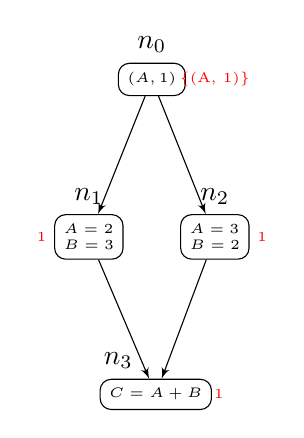
\begin{tikzpicture}[node distance = 2cm, auto, every text node part/.style={align=left}]
            % Place nodes
            \node [block, label=above:$n_0$] (n0) {$(A, 1)$};
            \node [value, right of=n0, node distance=0.8cm] (s0) {\{(A, 1)\}};
            \node [block, below of=n0, label=above:$n_1$, xshift=-0.8cm] (n1) {$A = 2$\\$B = 3$};
            \node [value, left of=n1, node distance=0.6cm] (s1) {1};
            \node [block, below of=n0, label=above:$n_2$, xshift=0.8cm] (n2) {$A = 3$\\$B = 2$};
            \node [value, right of=n2, node distance=0.6cm] (s2) {1};
            \node [block, below of=n1, label=130:$n_3$, xshift=0.85cm] (n3) {$C = A + B$};
            \node [value, right of=n3, node distance=0.8cm] (s3) {1};
            % Draw edges
            \path [line] (n0) -- (n1);
            \path [line] (n0) -- (n2);
            \path [line] (n1) -- (n3);
            \path [line] (n2) -- (n3);
            \end{tikzpicture}
        \end{center}
    \end{column}
  \end{columns}
\end{frame}

\begin{frame}
  \frametitle{Iteration Step}
  \begin{columns}[onlytextwidth]
    \begin{column}{0.55\textwidth}
      Visit nodes other than $n_0$ in order $v_1, v_2, ...$, for each visited node $n$, set \\
      \begin{equation*}
        B[n] = \bigwedge_{p \in PRED(n)} f_n(B[p])
      \end{equation*}

      \alert{Conditions} of the sequence($v_1, v_2, ...$):
      \begin{itemize}
      \item If a node doesn't satisfy the equation above, it should be visited again.
      \item If all nodes satisfy the equation, the sequence eventually end.
      \end{itemize}

      \only<1>{
        Example: \alert{$n_2, n_1, n_3, n_2, n_3$}
      }

    \end{column}

    \begin{column}{0.45\textwidth}
      \begin{center}
        \only<1>{
          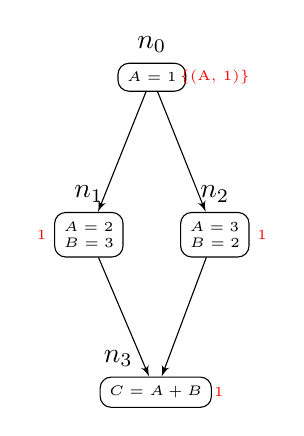
\begin{tikzpicture}[node distance = 2cm, auto, every text node part/.style={align=left}]
            % Place nodes
            \node [block, label=above:$n_0$] (n0) {$A = 1$};
            \node [value, right of=n0, node distance=0.8cm] (s0) {\{(A, 1)\}};
            \node [block, below of=n0, label=above:$n_1$, xshift=-0.8cm] (n1) {$A = 2$\\$B = 3$};
            \node [value, left of=n1, node distance=0.6cm] (s1) {1};
            \node [block, below of=n0, label=above:$n_2$, xshift=0.8cm] (n2) {$A = 3$\\$B = 2$};
            \node [value, right of=n2, node distance=0.6cm] (s2) {1};
            \node [block, below of=n1, label=130:$n_3$, xshift=0.85cm] (n3) {$C = A + B$};
            \node [value, right of=n3, node distance=0.8cm] (s3) {1};
            % Draw edges
            \path [line] (n0) -- (n1);
            \path [line] (n0) -- (n2);
            \path [line] (n1) -- (n3);
            \path [line] (n2) -- (n3);
          \end{tikzpicture}
        }
        \only<2>{
          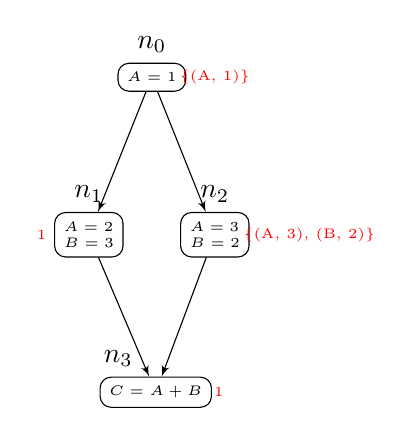
\begin{tikzpicture}[node distance = 2cm, auto, every text node part/.style={align=left}]
            % Place nodes
            \node [block, label=above:$n_0$] (n0) {$A = 1$};
            \node [value, right of=n0, node distance=0.8cm] (s0) {\{(A, 1)\}};
            \node [block, below of=n0, label=above:$n_1$, xshift=-0.8cm] (n1) {$A = 2$\\$B = 3$};
            \node [value, left of=n1, node distance=0.6cm] (s1) {1};
            \node [block, below of=n0, label=above:$n_2$, xshift=0.8cm] (n2) {$A = 3$\\$B = 2$};
            \node [value, right of=n2, node distance=1.2cm] (s2) {\{(A, 3), (B, 2)\}};
            \node [block, below of=n1, label=130:$n_3$, xshift=0.85cm] (n3) {$C = A + B$};
            \node [value, right of=n3, node distance=0.8cm] (s3) {1};
            % Draw edges
            \path [line] (n0) -- (n1);
            \path [line] (n0) -- (n2);
            \path [line] (n1) -- (n3);
            \path [line] (n2) -- (n3);
          \end{tikzpicture}

          \alert{$n_2$}, $n_1, n_3, n_2, n_3$
        }
        \only<3>{
          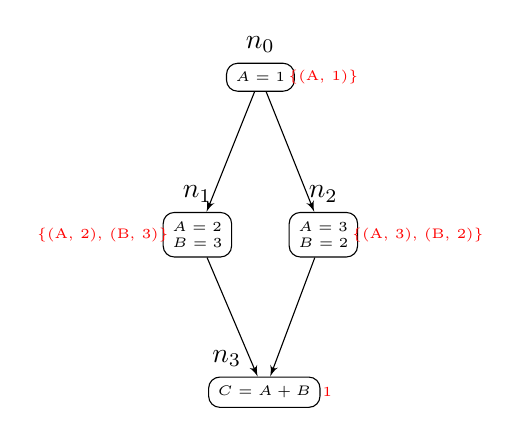
\begin{tikzpicture}[node distance = 2cm, auto, every text node part/.style={align=left}]
            % Place nodes
            \node [block, label=above:$n_0$] (n0) {$A = 1$};
            \node [value, right of=n0, node distance=0.8cm] (s0) {\{(A, 1)\}};
            \node [block, below of=n0, label=above:$n_1$, xshift=-0.8cm] (n1) {$A = 2$\\$B = 3$};
            \node [value, left of=n1, node distance=1.2cm] (s1) {\{(A, 2), (B, 3)\}};
            \node [block, below of=n0, label=above:$n_2$, xshift=0.8cm] (n2) {$A = 3$\\$B = 2$};
            \node [value, right of=n2, node distance=1.2cm] (s2) {\{(A, 3), (B, 2)\}};
            \node [block, below of=n1, label=130:$n_3$, xshift=0.85cm] (n3) {$C = A + B$};
            \node [value, right of=n3, node distance=0.8cm] (s3) {1};
            % Draw edges
            \path [line] (n0) -- (n1);
            \path [line] (n0) -- (n2);
            \path [line] (n1) -- (n3);
            \path [line] (n2) -- (n3);
          \end{tikzpicture}

          $n_2$, \alert{$n_1$}, $n_3, n_2, n_3$
        }
        \only<4>{
          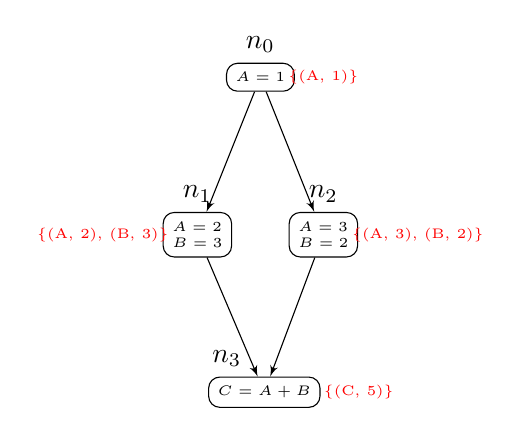
\begin{tikzpicture}[node distance = 2cm, auto, every text node part/.style={align=left}]
            % Place nodes
            \node [block, label=above:$n_0$] (n0) {$A = 1$};
            \node [value, right of=n0, node distance=0.8cm] (s0) {\{(A, 1)\}};
            \node [block, below of=n0, label=above:$n_1$, xshift=-0.8cm] (n1) {$A = 2$\\$B = 3$};
            \node [value, left of=n1, node distance=1.2cm] (s1) {\{(A, 2), (B, 3)\}};
            \node [block, below of=n0, label=above:$n_2$, xshift=0.8cm] (n2) {$A = 3$\\$B = 2$};
            \node [value, right of=n2, node distance=1.2cm] (s2) {\{(A, 3), (B, 2)\}};
            \node [block, below of=n1, label=130:$n_3$, xshift=0.85cm] (n3) {$C = A + B$};
            \node [value, right of=n3, node distance=1.2cm] (s3) {\{(C, 5)\}};
            % Draw edges
            \path [line] (n0) -- (n1);
            \path [line] (n0) -- (n2);
            \path [line] (n1) -- (n3);
            \path [line] (n2) -- (n3);
          \end{tikzpicture}

          $n_2$, $n_1$, \alert{$n_3$}, $n_2, n_3$ \\
          \textit{B[n] stablize now}
        }
      \end{center}
    \end{column}
  \end{columns}
\end{frame}

\subsection{Step 3}

\begin{frame}
  \frametitle{A Variant of Kildall's Algorithm - Final Step}
  \begin{itemize}
  \item \textit{Final Step}. Set \\
    \begin{equation*}
      H[n] =
      \begin{cases}
        0 & \text{if } n = n_0\\
        \bigwedge_{p \in PRED(n)} B[p] & otherwise
      \end{cases}
    \end{equation*}
  \end{itemize}
\end{frame}

%%%%%%%%%%%%%%%%%%%%%%%%%%%%%%%%%%%%%%%%%%%%%%%%%%%%%%%%%%%%%%%
% 5. Undecidability
%%%%%%%%%%%%%%%%%%%%%%%%%%%%%%%%%%%%%%%%%%%%%%%%%%%%%%%%%%%%%%%
\section{Undecidability of MOP Problem for frameworks} % (fold)
\label{sec:undecidability}

% section undecidability (end)
\begin{frame}[fragile]
    \frametitle{Example usage of blocks and columns}
    \begin{columns}
        \begin{column}{0.5\textwidth}
            \begin{block}{Block 1}
                \begin{itemize}
                    \item<1> 1
                    \item<2> 2
                    \item<3> 3
                \end{itemize}
            \end{block}
        \end{column}
        \begin{column}{0.5\textwidth}
            \begin{block}{Block 2}
                \begin{itemize}
                    \item<4> b
                    \item<5> b
                    \item<6> b
                \end{itemize}
            \end{block}
        \end{column}
    \end{columns}
\end{frame}
\end{document}
